\section{Function objects}
\subsection{Introduction}
\begin{frame}
  \frametitle{Function objects}
  \begin{itemize}
  \item defined in \texttt{<functional>}
  \item[]
  \item comparison criteria
  \item[]
  \item predicates (functions returning \texttt{bool})
  \item[]
  \item arithmetic operations
  \end{itemize}
\end{frame}
\begin{frame}
  \frametitle{Predicates}
  \centering
  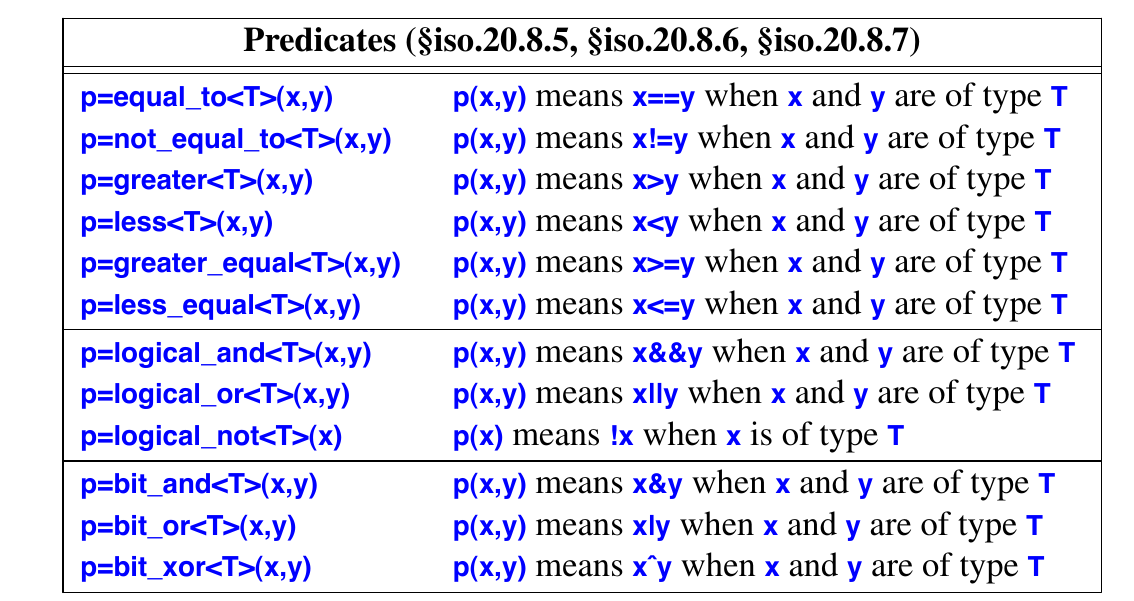
\includegraphics[width=0.8\textwidth]{img/predicates.png}
\end{frame}
\begin{frame}
  \frametitle{Arithmetic operations}
  \centering
  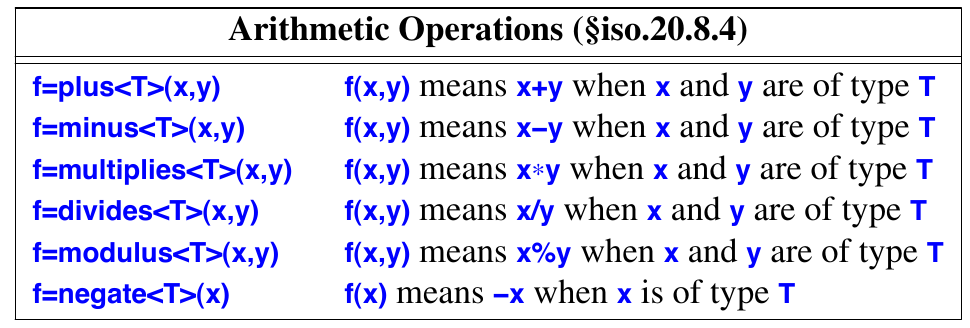
\includegraphics[width=0.8\textwidth]{img/arithmetic.png}
\end{frame}

\subsection{Examples}
\begin{frame}[fragile]
  \frametitle{Decreasing sort}
\begin{lstlisting}
#include <algorithm>
#include <vector>
#include <functional>
  
int main(){
  std::vector<double> v1;
  ...
  std::sort(v1.begin(), v1.end(),
            std::greater<double>{});
}
\end{lstlisting}
\end{frame}

\begin{frame}[fragile]
  \frametitle{My comparison}
\begin{lstlisting}
#include <algorithm>
#include <vector>
  
template <typename num>
struct my_comparison{
  bool operator()(const num& a, const num& b) { return a > b;}
};
  
int main(){
  std::vector<double> v1;
  ...
  std::sort(v1.begin(), v1.end(),
            my_comparison<double>{});
}
\end{lstlisting}
\end{frame}

\begin{frame}[fragile]
  \frametitle{Lambda}
\begin{lstlisting}
#include <algorithm>
#include <vector>

int main(){
  std::vector<double> v1;
  ...
  std::sort(v1.begin(), v1.end(),
           [](const auto& a, const auto& b)
              { return a>b; } );
}
\end{lstlisting}
\end{frame}
